\documentclass{IOS-Book-Article}
\usepackage[utf8]{inputenc}
\usepackage{graphicx}
\usepackage{framed}

\def\hb{\hbox to 11.5 cm{}}

\newcommand{\sembrack}[1]{[\![#1]\!]}
\newcommand{\subex}[2]{#1_{#2}}
\newcommand{\commentOut}[1]{}
\newcommand{\eop}[1]{\mbox{\textsl{#1}}}
\newcommand{\ttop}[1]{\mbox{\texttt{#1}}}

\newcommand{\bequ}{\begin{quote}}
\newcommand{\enqu}{\end{quote}}
\newcommand{\bece}{\begin{center}}
\newcommand{\ence}{\end{center}}

\newenvironment{compactitem}{\begin{itemize}}{\end{itemize}}

\begin{document}

\pagestyle{headings}
\def\thepage{}
\begin{frontmatter}              % The preamble begins here.

\title{An End-to-End Pipeline from Law Text to Logical Formulas}

\markboth{}{August 2022\hb}

\author[A]{Aarne Ranta}
\author[B]{Inari Listenmaa}
\author[C]{Jerrold Soh}
\author[D]{Meng Weng Wong}

\address[A]{
  Department of Computer Science and Engineering,
  Chalmers University of Technology and University of Gothenburg,
  aarne.ranta@cse.gu.se
  }
\address[B]{SMU and Digital Grammars}
\address[C]{SMU}
\address[D]{SMU}

\begin{abstract}
This paper describes an experimental pipeline starting from ordinary English law text, parsing it with a formal grammar, and converting it to logical formulas via a series of structural representations.
The goal is to see how to cover the full pipeline with a sequence of well-understood rule-based steps.
The approach is outside-in: we wanted to deliver some output from day 1, and refined it as we went on.
Thus it is a rule-based robust approach.
%%
The law text addressed is one chapter of law of Singapore, Part 6A of the Personal Data Protection Act 2012.
While more work is needed to port the method to other law texts, we believe to have achieved a reusable modular structure, as well as some reusable code, for a more general pipeline.
The pipeline includes some new methods and concepts, in particular, annotation-based grammar writing and an assemply logic for two-dimensional spreadsheet representations.
The code is available as open source.
\end{abstract}


\begin{keyword}
parsing law text
\end{keyword}
\end{frontmatter}
\markboth{August 2022\hb}{August 2022\hb}

%\maketitle




\section{Introduction}

Computational Law is an attempt to represent laws as computer programs.
Such programs can be used in expert systems, whose users can find out "what the law says" in different situations by posing explicit, concrete questions.
Some such systems are already in use, without even being called with that name.
For example, under the Covid-19 pandemic, travellers entering Singapore had to fill out web questionnaires about their country of origin, travel dates, and health data, and got an automatic answer telling them if they are allowed to enter and what test and quarantine plans they had to follow.

Setting up the Covid immigration system was a response to an emergency situation, where it would save work as possibly millions of people would be interested in entering the country, and their requests had to be treated efficiently.
The rules were, moreover, quite straightforward and unambiguous even if complex, and created in a time when web-based services were a normal way to organize things.
The situation is very different when it comes to laws in general: they may have a tradition of hundreds of years, so that decisions must be made by combining rules from different documents, which may seemingly contradict each othet and often be ambiguous.
Lawyers are needed to interpret them for laymen, case by case.
Lawyers are naturally also needed if laws are to be converted to expert systems.

The CCLAW project at Singapore Management University (SMU), School of Law, aims to develop technology that enables all laws of Singapore to be converted into computer systems.
The project uses natural language processing and theorem proving techniques, in particular, computational grammars and symbolic logics.
Many of the techniques are based on earlier work in computational law, but the ambition is somewhat different and more practical than in many other projects.
Thus the goal is to deal with the law as a whole, rather than selected and re-engineered fragments tailored to fit given methods.
The technology is also intended to leave room for a human in the loop: whenever the automated methods fail to give an unambiguous answer, a human lawyer can easily help it to take the decisive steps.
At the same time, the input required from the lawyer is reduced to the minimum, so that the routine coding work is carried out by the system.

From the technology point of view, CCLAW is building a classical pipeline where a parser converts a text to a formal representation, which is then converted to a set of logical formulas, for which an inference system exists or is developed.
In addition to the traditional components (syntax trees and logical formulas), the pipeline contains an intermediate spreadsheet representation of texts.
The spreadsheets aim to make the structure of the text explicit in a way that is readily accessible to lawyers, unlike syntax trees and formulas, which require training in formal logic and language theory.

The starting point of the project presented in this paper was a system consisting of \textbf{spreadsheets} and their translation to logical formulas.
The cells of the spreasheet were natural language expressions, which were parsed into syntax trees with the help of a grammar.
What was missing from the complete pipeline from text to logic was the conversion from the original text to spreadsheets.
This step was made manually, and the focus of the projects was on the later parts of the pipeline.
Thus the main contribution of the present paper is to define an automated conversion of texts to spreadsheets.
The first part of this is a grammar that parses texts to abstract syntax trees.
The second part is a conversion to a new intermediate representation between syntax trees, spreadsheets, and logic.
We call this representation \textbf{assembly logic}, in analogy to assembly languages in compilers, if we think of spreadsheets and logics as "machine languages", whose long distance to the source language is bridged by the assembly language.

Figure~\ref{pipeline} shows the complete pipeline, and Figure~\ref{pipeline-ex} shows an example of a text at different stages through the pipeline.

\begin{figure}
 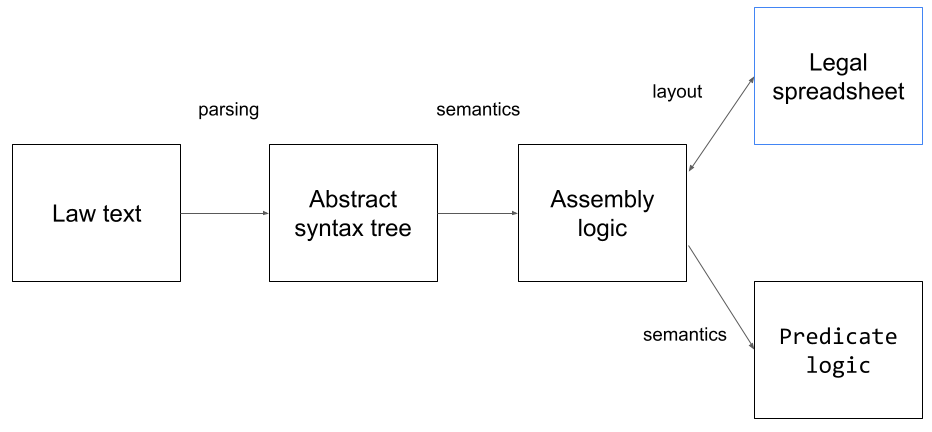
\includegraphics[width=0.8\textwidth]{pipeline.png}
\caption{The pipeline.}
\label{pipeline}
\end{figure}

\begin{figure}
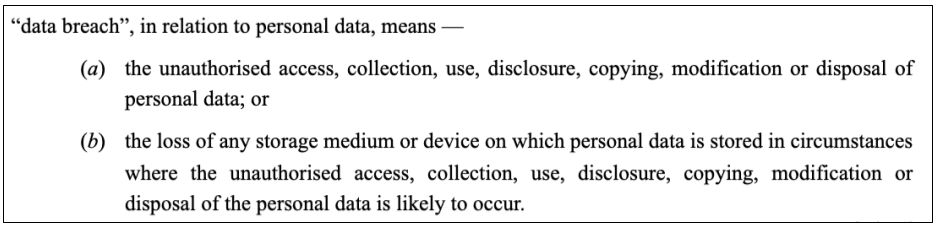
\includegraphics[width=0.8\textwidth]{text.png}
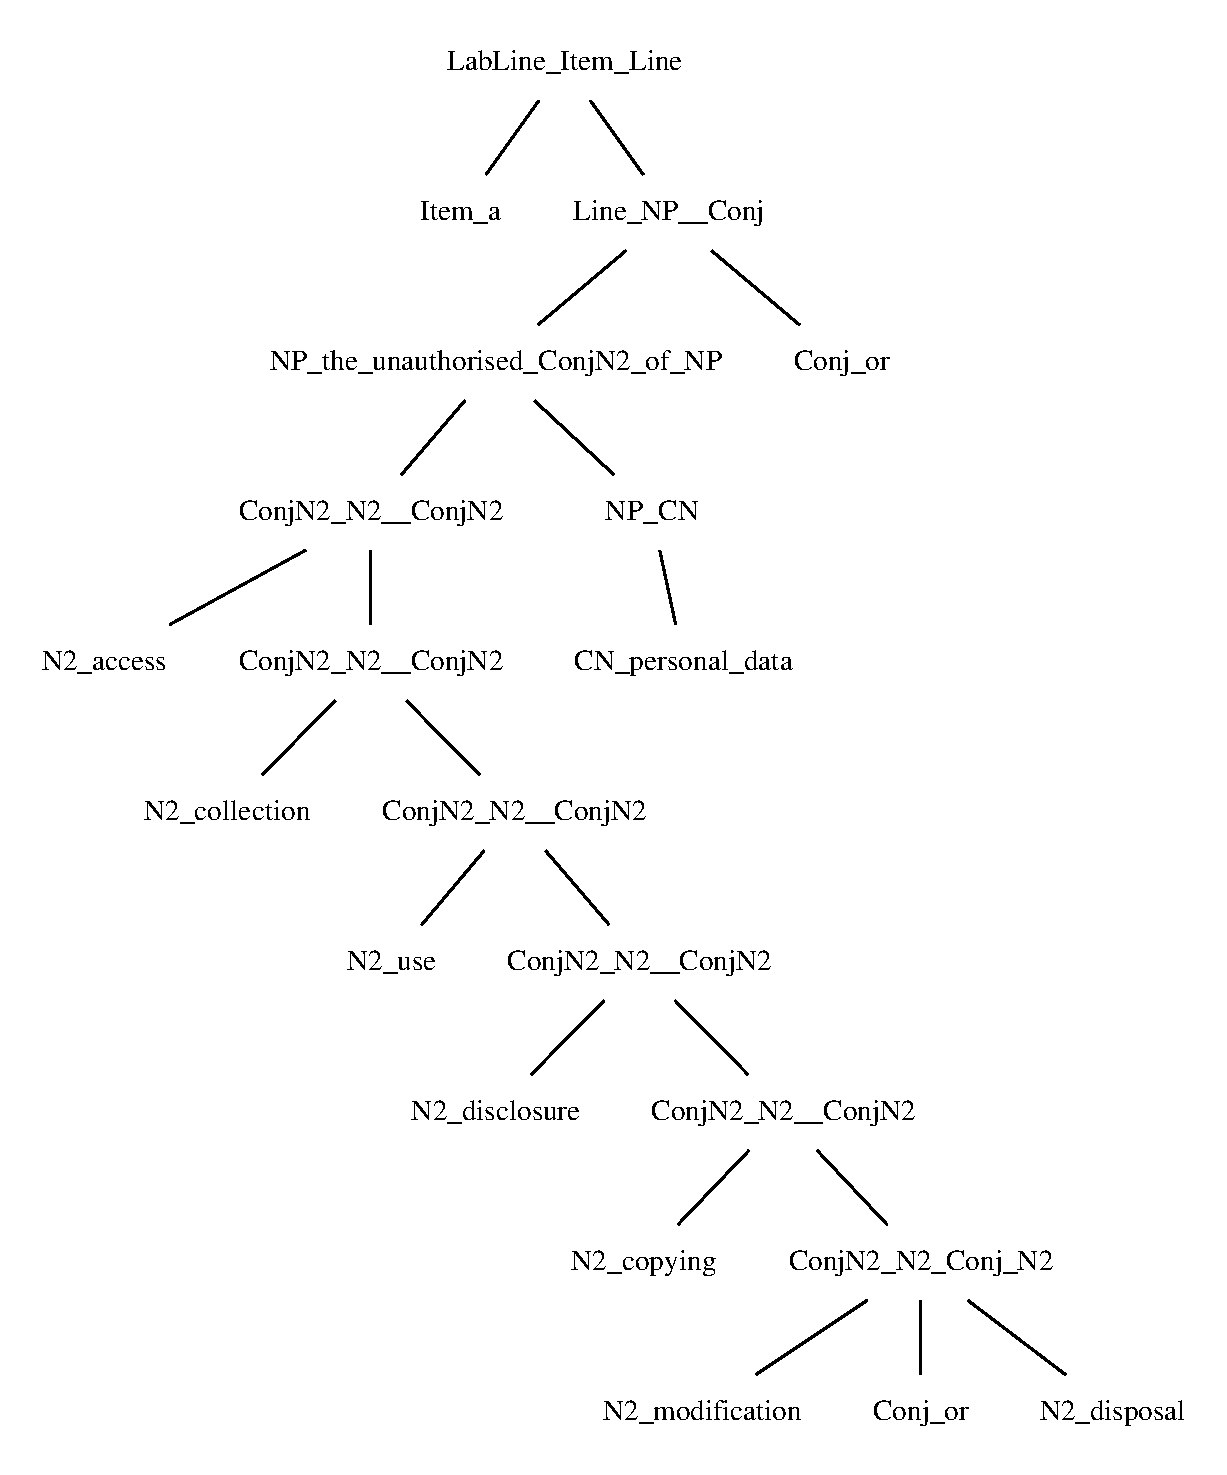
\includegraphics[width=0.4\textwidth]{tree.eps}
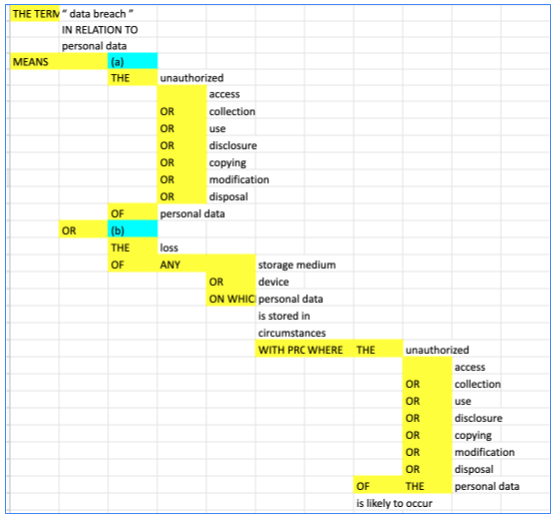
\includegraphics[width=0.6\textwidth]{assembly.png}
\small
\begin{verbatim}
![X]:(data_breach(X) & ?[Y]:(personal_data(Y) & IN_RELATION_TO(X,Y)) <=>
(personal_data(X) & ?[Y]:((access(Y,X) | collection(Y,X) | use(Y,X) |
disclosure(Y,X) | copying(Y,X) | modification(Y,X) | disposal(Y,X)) &
unauthorized(Y))) | (((storage_medium(X) | device(X)) & (personal_data(X) &
?[Y]:((circumstances(Y) & (((unauthorized(Y) & (access(Y) | collection(Y) |
use(Y) | disclosure(Y) | copying(Y) | modification(Y) | disposal(Y))) &
is_likely_to_occur(Y))) & is_stored_in(X,Y)))) & loss(X))))
\end{verbatim}
\normalsize
\caption{An example through the pipeline: text, abstract syntax tree (of the second line), spreadsheet, and formula in TPTP notation.
TODO (AR): the TPTP formula is not quite correct - I will have to fix the semantics.
}
\label{pipeline-ex}
\end{figure}


\section{Justifications for why GF and not the initial CFG}

(TODO: merge this section into appropriate section later)

\subsection{Comparison to Context-Free Grammars}

The first step from the annotation is to generate a context-free grammar (CFG, \cite{chomsky-1956}). On the first look, the use of GF seems to need justification, given that
\begin{enumerate}
\item[a)] the initially produced CFG perfectly describes the original document; and
\item[b)] CFGs are widely used in all branches of computer science, whereas GF is comes with a steeper learning curve.
\end{enumerate}

So why the extra step of going to a more expressive\footnote{GF is equivalent to Parallel Multiple Context-Free Grammars \cite{seki-al-1991}}, but less known formalism?

\paragraph{Abstract representations are not created equal}
While the initial CFG faithfully captures the original text, we must consider the larger context of this grammar.
The initial grammar produces the strings `to \emph{carry} out the deal`, `Acme \emph{carries} out the deal`), but their grammatical correctness is rather an accident.
The CFG doesn't know what verb conjugation and agreement are---it only knows strings, and in order to output these examples correctly, it needs to have a separate rule for how to handle \texttt{carry} and \texttt{carries}. If we translate this CFG naively into logical predicates, we will get a different predicate for each inflection form. This means that the further applications, such as automated theorem provers, will lose all connection between `Acme \emph{carries} out the deal` and `Acme doesn't \emph{carry} out the deal`.

In contrast, the GF grammar has a higher level of abstraction, and it knows all about the English phrasal verb \emph{carry out}: how the verb is conjugated, and how the particle \emph{out} behaves with different objects (\emph{carry out the deal} vs. \emph{carry it out}). This representation gives us two immediate benefits over the CFG:
\begin{enumerate}
\item The grammar is more general, and can be used to parse unseen text with much smaller additions compared to the CFG; and
\item No redundancy needed in grammar rules: logical predicates can be produced from the same grammar that is used for parsing.
\end{enumerate}

For these reasons, we consider it worthwile to convert the initial CFG into a full GF grammar, even with the manual effort it takes.


\section{Building the grammar}

Parsing the text is performed by the Grammatical Framework (GF) software \cite{ranta-2011}.
The parser is driven by a grammar, which specifies a relation between strings and abstract syntax trees.
In typical GF applications, abstract syntax trees are processed further, usually in translations to other languages but also in logical semantics.

GF grammars are usually written by hand, to guarantee a precise correspondance to desired abstract syntax trees.
The process is helped by GF's module system and extensive libraries, which reduce the need of manual work to the minimum.
This is particularly useful in the most typical application of GF, Controlled Natural Language (CNL) \cite{fuchs-al-2008,angelov-ranta-2009}.
In such applications, the language can be made to follow grammar rules defined in the GF Resource Grammar Library (RGL, \cite{ranta-2009}).

However, the RGL does not cover all the constructs in Singaporean law text, which means that some grammar writing needs to be done from scratch.
In particular, the text contains indented lists, paragraph numbers, and references, which significant for the logical structure and which we wanted to capture by the parser.
In order to make sure to capture everything, we started grammar writing in a data-driven, top-down way, starting from entire lines of text and going forward by stepwise refinements of the grammar rules.

The most efficient way to produce the grammar turned out to be a semi-automatic method consisting of manual annotations from which a script generated GF rules.
Figure~\ref{grammar-gen} shows an example of a line of a text, the annotations added to it, and the resulting grammar rules.


\begin{figure}
 \begin{framed}
\bequ
\textbf{A line in the text:}
\bequ
\textit{Item (2) without limiting subsection Ref (1)(a), a CN data breach is deemed to VP result in significant harm to an individual —}
\enqu
\textbf{The line annotated with marks for terminals} (\verb6#6) \textbf{and nonterminals} (\verb6*6):
\bequ
\begin{verbatim}
*Item (2) #without #limiting #subsection *Ref (1)(a) #,
#a *CN data breach #is #deemed #to
*VP result in significant harm to an individual #—
\end{verbatim}
\enqu
\textbf{Grammar rules derived by the script:}
\bequ
\begin{verbatim}
Line ::= Item "without" "limiting" "subsection" Ref ","
         "a" CN "is" "deemed" "to" VP "-" ;
Item ::= "(2)" ;
Ref  ::= "(1)(a)" ;
CN   ::= "data" "breach" ;
VP   ::= "result" "in" "significant"
         "harm" "to" "an" "individual" ;
\end{verbatim}
\enqu
\textbf{The last of the grammar rules manually edited by step-wise refinements:}
\bequ
\begin{verbatim}
VP2 ::= "result" "in" NP ;
NP  ::= "significant" "harm" "to" NP ;
NP  ::= "an" CN ;
CN  ::= "individual" ;
\end{verbatim}
\enqu
\textbf{Abstract syntax functions in the resulting GF grammar:}
\bequ
\begin{verbatim}
fun VP2_result_in : VP2 ;
fun CN_significant_harm_to_NP : NP -> CN ;
fun NP_an_CN : CN -> NP ;
fun CN_individual : CN ;
\end{verbatim}
\enqu
\enqu
\end{framed}
\caption{The grammar extraction process.}
\label{grammar-gen}
\end{figure}

The grammar produced by the script is a BNF (context-free) grammar, in a notation that can be used in GF as it is.
Internally, GF adds to each rule abstract syntax functions, whose names are derived from items in the rule itself.
Full GF is more expressive and more abstract than BNF.
In the example of Figure~\ref{grammar-gen}, the full power can be used to merge together the function \verb6CN_individual6 with another derived function \verb6CN_individuals6, to a single function that covers both the singular and the plural form of the noun.
Similarly, the rules \verb6NP_an_CN6 can be merged with \verb6NP_a_CN6.
An advantage, in addition to getting fewer rules, is that the choice of the sinular and the plural, or \textit{a} vs.\ \textit{an}, can then be made precisely depending on the context.



\section{Assembly logic and spreadsheets}

We implemented spreadsheets with a recursive datatype \verb6Box6, where a box consists of a header and cells, where each cell is a box with a title.
This structure supports compositional conversion from a tree-like representation, but also rendering as tab-separated files, which can be read into spreadsheet editors.
Figure~\ref{assembly} shows this type, together with the other concepts related to spreadsheets.

\begin{figure}
  \begin{framed}
  \bequ
  \textbf{The recursive Haskell datatype for spreadsheets:}
 \bequ
\begin{verbatim}
data Box = Box {
   header :: String,
   cells :: [(String, Box)]
  }
\end{verbatim}
 \enqu

 \textbf{Some assembly logic constructors:}
 \bequ
\begin{verbatim}
data Cat =
  CProp | CSet | CInd | -- ...

data Formula =
    Atomic Cat Atom
  | Conjunction Cat ConjWord [Formula]
  | Implication Formula Formula
  | Conditional Formula Formula     -- reverse implication
  | Quantification String Formula   -- quantifier + domain
\end{verbatim}
 \enqu

 \textbf{Semantics of abstract syntax trees in the assembly logic:}
 \bequ
\begin{verbatim}
iNP :: Env -> GNP -> Formula
iNP env np = case np of
  GNP_any_CN cn -> Quantification "ANY" (iCN env cn)
  GNP_each_CN cn -> Quantification "EACH" (iCN env cn)
  -- ...
  _ -> Atomic CInd (lin env (gf np))
\end{verbatim}
 \enqu

 \textbf{Conversions from assembly logic to spreadsheets:}
 \bequ
\begin{verbatim}
formula2box :: Formula -> Box
formula2box formula = case formula of
  Atomic _ a  -> atomBox a
  Implication f g -> ifBox [formula2box f] [formula2box g]
  Quantification s f -> leftsideBox s [formula2box f]
\end{verbatim}
 \enqu
 \enqu
   \end{framed}
 \caption{Data structures and conversions related to spreadsheet and the assembly logic.
 }
\label{assembly}
\end{figure}

Notice that the ultimate unit of semantic interpretation is a paragraph consisting of several lines.
This is the case, for instance with the example in Figure~\ref{pipeline-ex}.
In the current implementation, the parser reads the document line by line, and a separate process is used for segmenting groups of lines into paragraphs.
The reason for this set-up is purely practical: semantic units can be arbitrarily long sequences of lines, and the parser may get slow in such cases.




\section{Interpretation in predicate logic}

The pipeline in Figure~\ref{pipeline} branches from Assembly Logic to two directions: to spreadsheets, as described in the previous section, and to predicate logic, to be discussed here.
The predicate logic step itself is divided to two phases:
\begin{enumerate}
\item Assembly logic is mapped into a many-sorted logic with Russell iota terms.
\item The many-sorted logic is mapped into ordinary predicate logic and rendered in the TPTP notation.
\end{enumerate}
The many-sorted logic is chosen because of its better support of compositional translation.
Thus quanfication expressed by noun phrases (such as \textit{any storage medium}) are compositionally interpreted as quantifiers with sorts, instead of dividing them into unsorted quantiers and sort predicates.
The sorts are eliminated as a part of the conversion from many-sorted to ordinary logic.

Even more crucially, anaphoric expressions (such as \textit{that organization}) are interpreted as definite descriptions formalized as iota terms.
These iota terms are eliminated in a pass that looks for non-iota terms in their context of use.
Figure~\ref{anaphora} shows an examples of this, showing thestructure of ``donkey sentences'' well-known in linguistic literature (\textit{if a man owns a donkey he beats it}) \cite{geach-1962,kamp-1981}
Such a sentence has an existential quantifier in the antecedent, and a pronoun or definite desctiption referring to it in the succedent.
To express this reference in ordinary predicate logic, the existential quantifier is changed into a universal with a wide scope of the implication.

 \begin{figure}
  \begin{framed}
  \bequ
  \textbf{A toy example of a ``donkey sentence'':}
  \bequ
 \textit{if a notification is a data breach , the notification is affected}
 \enqu

 \textbf{Compositional interpretation in many-sorted logic with iota terms:}
 \[
(\exists x : \eop{notification})\eop{data\_breach}(x) \, \supset \, \eop{affected}(\iota(\eop{notification}))
\]

 \textbf{Conversions to ordinary predicate logic in TPTP notation:}
 \bequ
\begin{verbatim}
![X]:(notification(X) => data_breach(X) => affected(X))
\end{verbatim}
 \enqu
 \enqu
   \end{framed}
 \caption{Iota terms are eliminated via anaphora resolution.
 }
\label{anaphora}
\end{figure}

Donkey sentences are ubiquitous in law text, as in many other types of text.
To our surprise, also ``inverted donkey sentences'' occurred in our sample text --- ones in which the existential appears in the succedent and is referred to in the antecedent.
What makes this sound natural is that the whole implication appears in reverse: \textit{a man beats a donkey if he owns it}.
Figure~\ref{donkey}



\begin{figure}
 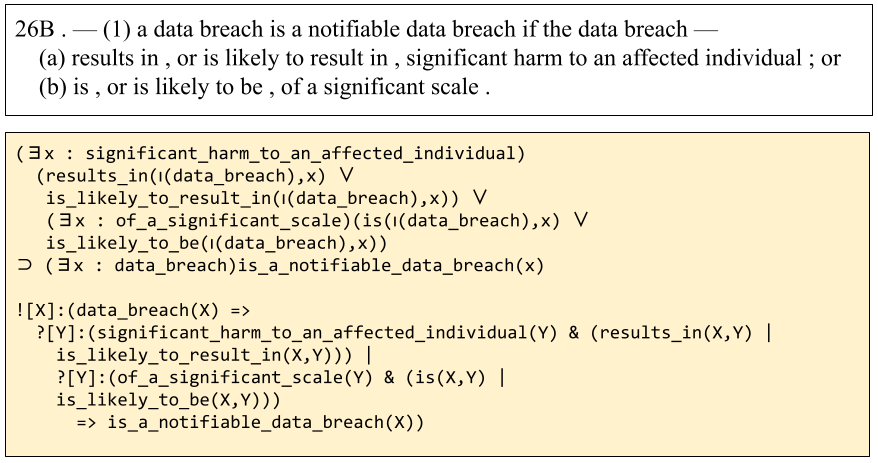
\includegraphics[width=0.96\textwidth]{anaphora.png}
\caption{An inverted donkey sentence from the actual law text.}
\label{donkey}
\end{figure}

\section{Results, evaluation, and future work}

Table~\ref{stats} shows some figures about the corpus used in this case study.

TODO (AR): At the time of writing, the final translation to logic fails for two logical units, and the logic rules require better verification.


\begin{table}
  \begin{tabular}{|l|r|}
\hline
lines & 66 \\
characters & 6154 \\
tokens & 1072 \\
unique tokens & 229 \\
tokens per line on average & 16 \\
tokens on the longest line & 56 \\
logical units & 46 \\
\hline
  \end{tabular}
  \caption{Statistics about Personal Data Protection Act (PDPA), Part 6A}
  \label{stats}
\end{table}

The most important tasks for future work are to link this pipeline with the previous work at CCLAW, which have much more precision and detail: the spreadsheets and the grammar of smaller units.

As regards spreadsheets, and in fact the interpretation in logic, the current experiment is simple-minded in the sense that it only looks at the document at hand.
The real spreasheets also take into account other documents that affect the interpretation, and show this information in the spreadsheets.

As for the grammar, the bulk of the work will be in the detailed structure of noun phrases and predicates that appear in single cells.
It also remains to see how much of the line and paragraph structures is already included in the grammar based on the sample, but the variation there can be expected to be numerically smaller.



\section{Conclusion}

\bibliographystyle{plain}
\bibliography{gf-bib}



\end{document}
